% Copyright 2026 Sreeram Anil
% SPDX-License-Identifier: CC-BY-4.0
% =============================================================================
%  Extended Kalman filter — classical Kalman family
% =============================================================================
\chapter{Extended Kalman Filter (EKF)}
\label{ch:ekf}

\section*{At a glance}
\begin{tabular}{@{}l>{\raggedright\arraybackslash}p{0.76\textwidth}@{}}
Family & classical Kalman \\
Header & \texttt{include/estkit/filters/ekf.hpp} \\
Registered name & \texttt{EKF} \\
State dimension & $n_x = 4$ (cell model) --- generic in $n_x, n_u, n_y$ \\
Cost per step & $\mathcal{O}(n_x^3 + n_x^2 n_y)$, $443$--$482$\,ns/step measured, no heap \\
Primary references & \cite{kalman1960,jazwinski1970,plett2004ekf3,bucyjoseph1968} \\
\end{tabular}

\section{Motivation and aerospace/BMS relevance}
The extended Kalman filter is the reference implementation of model-based state of charge
(SOC) estimation and the yardstick against which every other method in this report is
measured. Its appeal is entirely practical: it costs a handful of $n_x\times n_x$ matrix
products per sample, it needs no tuning beyond the noise covariances, and it produces a
covariance that a supervisory function can turn into a usable confidence interval --- exactly
what a certified battery management system (BMS) needs when it has to publish a
\emph{remaining energy} figure with a guaranteed margin.

Coulomb counting alone integrates the current sensor and
therefore integrates its bias; voltage inversion alone is
blind whenever the cell is loaded, because the ohmic and diffusion overpotentials swamp the
open-circuit voltage (OCV) signature. The EKF is the minimal estimator that fuses the two:
ampere-hour integration supplies the fast, smooth, drift-prone prediction, and the terminal
voltage supplies the slow, noisy, drift-free correction. Plett's three-part
paper~\cite{plett2004ekf1,plett2004ekf2,plett2004ekf3} established this structure for
lithium-polymer packs and it remains the industrial baseline.

For electric vertical take-off and landing (eVTOL) aircraft the stakes are higher than in
automotive use because there is no roadside: the reserve computation of the final approach
depends directly on the SOC estimate, and the C-rates during hover are three to five times
those of a road vehicle~\cite{yang2021evtol,fredericks2018vtol}, so the overpotential that
the model has to subtract from the measured voltage is large and strongly temperature
dependent. DO-311A~\cite{rtca2017do311a} requires the state-of-charge indication to be
substantiated; a filter that also reports $\mP$ makes that substantiation possible.

\section{Problem statement and assumptions}
The plant is a discrete-time nonlinear system with additive Gaussian noise,
\begin{align}
\vx_{k} &= f(\vx_{k-1}, \vu_{k-1}) + \vw_{k-1}, & \vw_k &\sim \N{\bm{0}}{\mQ_k}, \label{eq:ekf-proc}\\
\vy_{k} &= h(\vx_{k}, \vu_{k}) + \vv_{k},       & \vv_k &\sim \N{\bm{0}}{\mR_k}, \label{eq:ekf-meas}
\end{align}
where $\vx_k\in\real^{n_x}$ is the state, $\vu_k\in\real^{n_u}$ the (known, measured) input,
$\vy_k\in\real^{n_y}$ the measurement, $\vw_k$ and $\vv_k$ mutually independent white
sequences, $\mQ_k\in\real^{n_x\times n_x}$ and $\mR_k\in\real^{n_y\times n_y}$ their
covariances, and $f,h$ continuously differentiable. The filter maintains the first two
moments of the conditional density $p(\vx_k\mid \vy_{1:k})$: the estimate
$\xplus_k = \E{\vx_k \mid \vy_{1:k}}$ and the error covariance
$\Pplus_k = \E{(\vx_k-\xplus_k)(\vx_k-\xplus_k)^\T \mid \vy_{1:k}}$. The superscripts $^-$
and $^+$ denote the values before and after the measurement of step $k$ is used.

\begin{assumption}[Local linearity]\label{as:ekf-lin}
Over a region of the state space whose size is set by $\mP$, $f$ and $h$ are well
approximated by their first-order Taylor expansions about the current estimate.
\end{assumption}
Assumption~\ref{as:ekf-lin} is the only approximation the EKF makes, and every failure mode
observed in the benchmark can be traced back to it.

\section{Derivation}
Expand \eqref{eq:ekf-proc} about $\xplus_{k-1}$ and \eqref{eq:ekf-meas} about $\xminus_k$:
\begin{align}
f(\vx,\vu_{k-1}) &\approx f(\xplus_{k-1},\vu_{k-1}) + \mF_{k-1}\,(\vx - \xplus_{k-1}),
 & \mF_{k-1} &= \left.\frac{\partial f}{\partial \vx}\right|_{\xplus_{k-1},\vu_{k-1}}, \label{eq:ekf-F}\\
h(\vx,\vu_k) &\approx h(\xminus_{k},\vu_k) + \mH_{k}\,(\vx - \xminus_{k}),
 & \mH_{k} &= \left.\frac{\partial h}{\partial \vx}\right|_{\xminus_{k},\vu_k}. \label{eq:ekf-H}
\end{align}
$\mF_{k-1}\in\real^{n_x\times n_x}$ and $\mH_k\in\real^{n_y\times n_x}$ are the process and
measurement Jacobians. Substituting \eqref{eq:ekf-F} into \eqref{eq:ekf-proc} and taking the
first two moments gives the time update
\begin{align}
\xminus_k &= f(\xplus_{k-1}, \vu_{k-1}), \label{eq:ekf-tu-mean}\\
\Pminus_k &= \mF_{k-1}\Pplus_{k-1}\mF_{k-1}^\T + \mQ_{k-1}. \label{eq:ekf-tu-cov}
\end{align}
With \eqref{eq:ekf-H} the joint density of $(\vx_k,\vy_k)$ given $\vy_{1:k-1}$ is Gaussian
with cross-covariance $\Pminus_k\mH_k^\T$ and measurement covariance
\begin{equation}
\mS_k = \mH_k \Pminus_k \mH_k^\T + \mR_k \in\real^{n_y\times n_y}, \label{eq:ekf-S}
\end{equation}
the \emph{innovation covariance}. Conditioning a joint Gaussian (the standard Gaussian
conditioning lemma, e.g.~\cite[\S A.1]{sarkka2013}) yields
\begin{align}
\mK_k &= \Pminus_k \mH_k^\T \mS_k\inv \in \real^{n_x\times n_y}, \label{eq:ekf-K}\\
\xplus_k &= \xminus_k + \mK_k \underbrace{\left(\vy_k - h(\xminus_k,\vu_k)\right)}_{\text{innovation } \veps_k},
 \label{eq:ekf-mu}\\
\Pplus_k &= \left(\mI - \mK_k\mH_k\right)\Pminus_k. \label{eq:ekf-cu}
\end{align}
$\mK_k$ is the Kalman gain. Form \eqref{eq:ekf-cu} is a difference of two positive
semi-definite matrices and can lose symmetry or definiteness under round-off; the
implementation uses the algebraically equivalent Joseph form~\cite{bucyjoseph1968}
\begin{equation}
\Pplus_k = (\mI-\mK_k\mH_k)\Pminus_k(\mI-\mK_k\mH_k)^\T + \mK_k\mR_k\mK_k^\T,
\label{eq:ekf-joseph}
\end{equation}
which is a sum of two positive semi-definite terms and is therefore positive semi-definite
for \emph{any} gain $\mK_k$, not only the optimal one --- a property that matters when the
gain has been modified (robust weighting, fading memory, constraint projection).

For the linear case $f(\vx,\vu)=\mF\vx+\mG\vu$, $h(\vx,\vu)=\mH\vx$, equations
\eqref{eq:ekf-tu-mean}--\eqref{eq:ekf-cu} are exactly Kalman's original recursion and
$\xplus_k$ is the minimum-variance estimate among \emph{all} measurable functions of
$\vy_{1:k}$~\cite{kalman1960}. In the nonlinear case no optimality survives: the EKF is a
first-order approximation whose error is $\mathcal{O}(\norm{\vx-\xhat}^2)$ in the mean and
$\mathcal{O}(\norm{\vx-\xhat}^3)$ in the covariance, and it is known to be over-confident
precisely because \eqref{eq:ekf-S} ignores the variance contributed by the curvature of $h$
(the term the second-order filter of Chapter~\ref{ch:soekf} restores).

\section{Algorithm}
\begin{algorithm}[H]
\caption{EKF --- one sampling period}
\begin{algorithmic}[1]
\Require $\xplus_{k-1}, \Pplus_{k-1}, \vu_{k-1}, \vy_k, \vu_k$
\State \textbf{Time update:} $\mF \gets \partial f/\partial\vx |_{\xplus_{k-1},\vu_{k-1}}$
\State $\xminus_k \gets f(\xplus_{k-1},\vu_{k-1})$
\State $\Pminus_k \gets \mF\Pplus_{k-1}\mF^\T + \mQ$; symmetrise
\State \textbf{Predicted measurement:} $\yhat_k \gets h(\xminus_k,\vu_k)$
\State \textbf{Measurement update:} $\mH \gets \partial h/\partial\vx |_{\xminus_k,\vu_k}$
\State $\mS \gets \mH\Pminus_k\mH^\T + \mR$, \quad $\mK \gets \Pminus_k\mH^\T\mS\inv$
\State $\xplus_k \gets \xminus_k + \mK(\vy_k - \yhat_k)$
\State $\Pplus_k \gets (\mI-\mK\mH)\Pminus_k(\mI-\mK\mH)^\T + \mK\mR\mK^\T$; symmetrise
\State \textbf{if} constraints enabled \textbf{then} $\xplus_k \gets \Pi(\xplus_k)$
\Ensure $\xplus_k, \Pplus_k$
\end{algorithmic}
\end{algorithm}
$\Pi$ is the projection onto the physically feasible set ($\soc\in[-0.05,1.05]$,
$h\in[-1,1]$), the simplest of the constrained-filtering options surveyed
in~\cite{simon2010constraints}.

\section{Application to the battery model}
With $\vx=[\soc,v_1,v_2,h]^\T$, $\vu=[i,T]^\T$ and $y=v$ (Chapter~\ref{ch:ecm}), the
Jacobians are available in closed form, which is why the EKF is so cheap here:
\begin{equation}
\mF = \diag\!\left(1,\;a_1(T),\;a_2(T),\;a_h(i)\right), \qquad
\mH = \begin{bmatrix}\dfrac{\partial \ocv}{\partial \soc}(\soc,T) & -1 & -1 & M\end{bmatrix},
\label{eq:ekf-battery-jac}
\end{equation}
with $a_j(T)=\exp(-\dt/\tau_j(T))$, $a_h(i)=\exp(-|\eta(i) i \gamma \dt/(3600Q)|)$ and $M$
the hysteresis magnitude in volts. $\mF$ is diagonal: the four states are dynamically
decoupled and only the measurement couples them. The entire observability of $\soc$ rests on
the single entry $\partial\ocv/\partial\soc$, which for the NMC811/graphite cell used here
varies between $0.71$ and $0.93$\,V over the mission --- modest variation, but the
\emph{offset} of the tangent line drifts far more (Chapter~\ref{ch:lkf} quantifies this).

The process noise is built from the current-sensor specification,
$\mQ = \bm{b}\bm{b}^\T\sigma_i^2 + \diag(q_{\text{floor}}^2)$ with
$\bm{b}=\partial f/\partial i$, so that current noise enters through the same channel as the
current itself; $\mR = \sigma_v^2 + (R_0(T)\sigma_i)^2$ accounts for the fact that current
noise also feeds through the ohmic drop. Benchmark options: \code{joseph = true},
\code{apply\_constraints = true}, \code{q\_scale = r\_scale = 1} --- that is, no tuning at
all beyond the sensor data sheet.

\section{Implementation notes}
The covariance is symmetrised after both updates. The Joseph form costs one extra
$n_x\times n_x$ product but removes the only realistic route to an indefinite $\mP$ at
$n_x=4$. All memory is static: \code{sizeof(Ekf<EcmModel>)} is 4336\,bytes, dominated by the
241-point OCV table carried inside the model copy, not by the filter state (the filter itself
needs $n_x + n_x^2 + n_y^2 + n_x n_y = 25$ reals $=200$\,bytes in double).
The flop count per step is $\approx 2n_x^3 + 4n_x^2 n_y \approx 150$ multiply-accumulates for
the cell model, plus three exponentials in $f$; on a 200\,MHz Cortex-M7 with hardware
double precision this is well under \SI{10}{\micro\second}, i.e. below 0.1\,\% duty at
\SI{10}{\hertz}. In the \code{-DESTKIT\_FLOAT=ON} build the nominal steady-state RMSE is unchanged
at $0.06\,\%$ (and \texttt{aged\_cell} moves from $1.39$ to $1.48\,\%$); no covariance ever
lost positive definiteness. The peak
condition number of $\mP$ along the mission is $\approx 1.3\times10^6$, which is the number
to compare against $1/\varepsilon_{\text{float}}\approx 8\times 10^6$ when deciding whether a
factored implementation (Chapters~\ref{ch:srekf}, \ref{ch:udekf}) is needed.

\section{Benchmark results}
\input{tables/cell_EKF.tex}
\begin{figure}[H]\centering
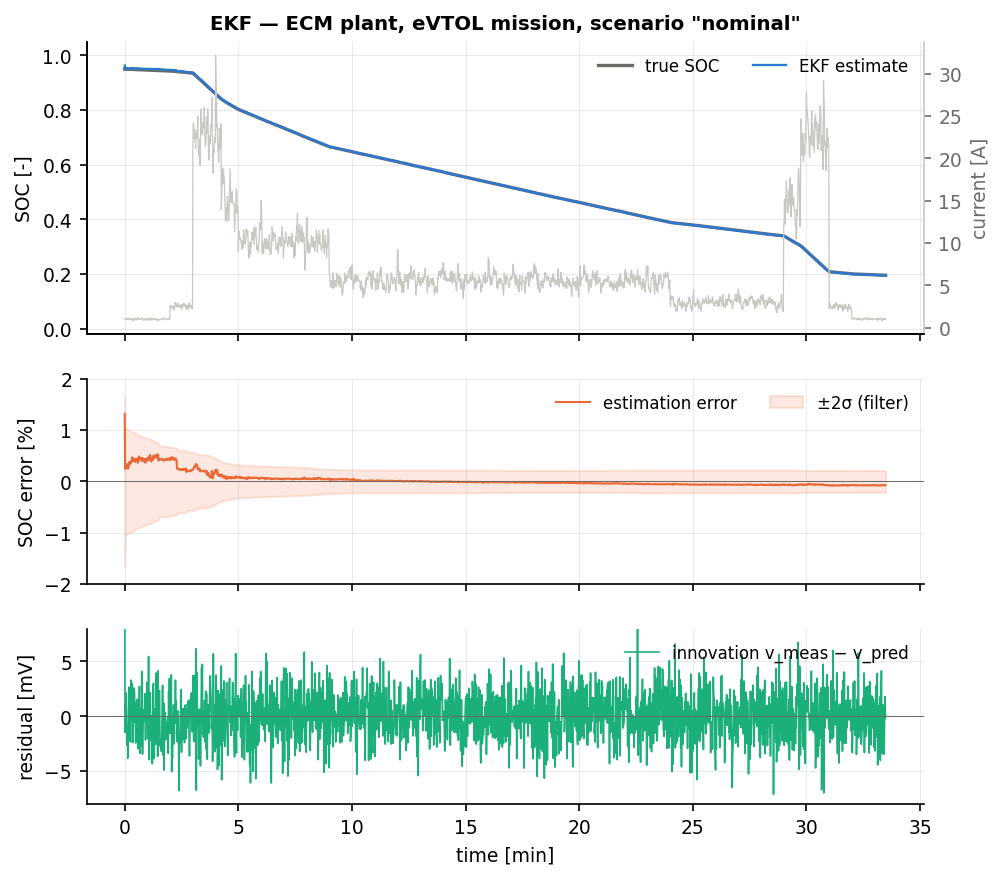
\includegraphics[width=\textwidth]{figures/cell_EKF_nominal.png}
\caption{EKF on the nominal eVTOL mission: true and estimated SOC (top), estimation error with the $\pm 2\sigma$ band when available (middle), voltage residual (bottom).}
\end{figure}
\begin{figure}[H]\centering
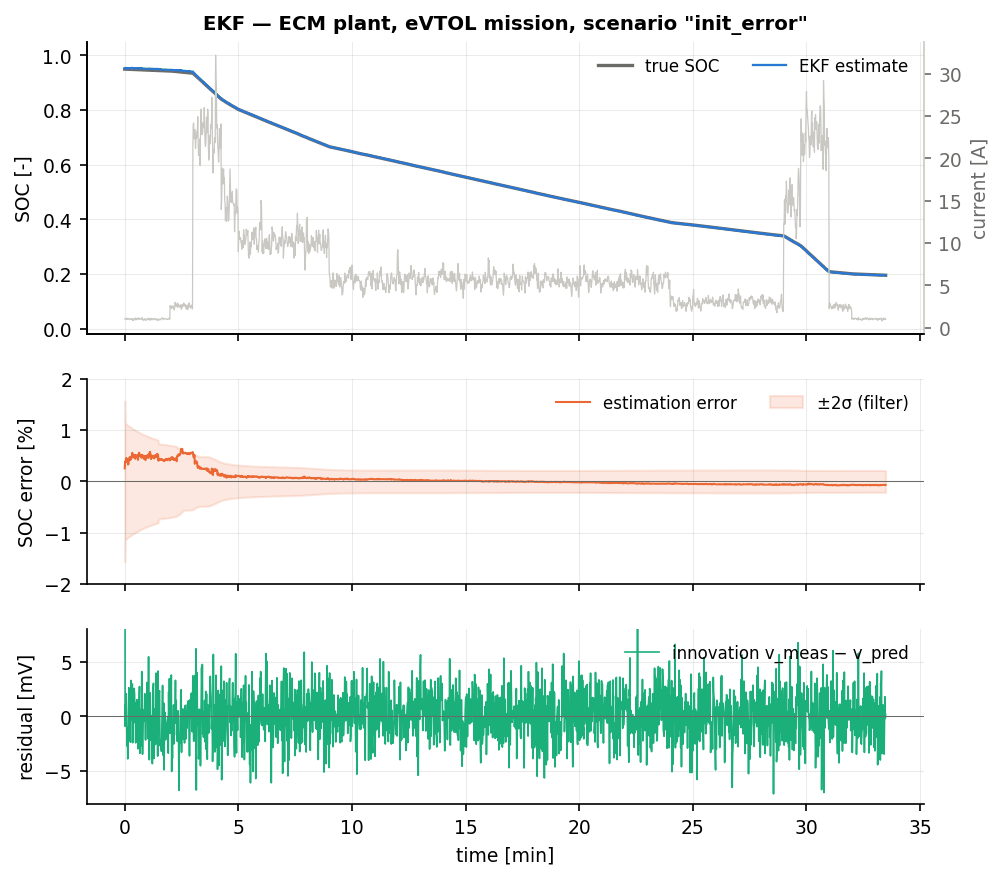
\includegraphics[width=\textwidth]{figures/cell_EKF_init_error.png}
\caption{EKF with a 35\,\% initial SOC error.}
\end{figure}
\begin{figure}[H]\centering
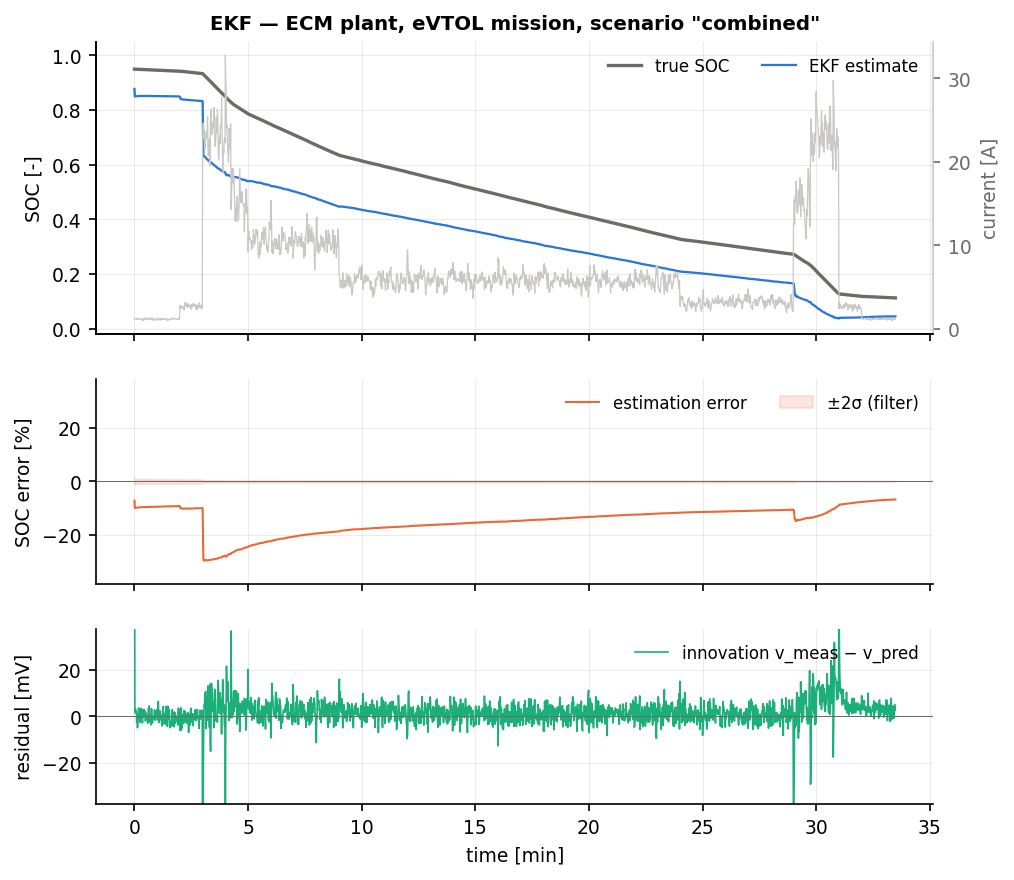
\includegraphics[width=\textwidth]{figures/cell_EKF_combined.png}
\caption{EKF on the \texttt{combined} scenario ($-25\,\%$ initial SOC error, $0.15$\,A current bias, $10\,\%$ capacity loss, $0^\circ$C): the covariance collapses after the first update and the estimate is locked in.}
\end{figure}

All numbers quoted here are three-seed means in per cent SOC, as printed in the table.

On the nominal eVTOL mission the EKF reaches $\text{RMSE} = 0.15\,\%$ over the whole run and
$0.05\,\%$ in steady state, with a voltage-residual RMSE of $0.79$\,mV --- essentially the
sensor noise floor ($\sigma_v = 2$\,mV, quantised at 1\,mV) --- and a maximum error of
$1.07\,\%$. The $-35\,\%$ initial SOC error is removed in a single sample
($t_{\text{conv}} = 0$\,s, $\text{RMSE}_{\text{ss}} = 0.05\,\%$): because the mission begins at
low current and $\Pminus_{\soc\soc} = 10^{-2}$ is four orders of magnitude larger than
$\mR/\mH^2\approx10^{-5}$, the first innovation of $0.28$\,V is almost entirely absorbed by
$\soc$. This is the behaviour that makes the EKF hard to beat on \emph{well-posed} problems and
it is worth stating explicitly: the local linearisation is not a handicap when the prior is
tight or the residual is small.

The failure modes are all consequences of Assumption~\ref{as:ekf-lin} plus the over-confidence
of \eqref{eq:ekf-S}. \texttt{current\_bias} ($0.25$\,A offset, $+2\,\%$ gain) settles at
$0.61\,\%$: the bias is unobservable from a single voltage measurement without an augmented
state, so the filter trades it against the OCV, exactly as predicted
by~\cite{zhao2017observability,lin2018sensorbias}. \texttt{aged\_cell} ($15\,\%$ capacity loss)
gives $1.52\,\%$ and \texttt{param\_mismatch} ($R_0$ at $70\,\%$, $R_1$ at $130\,\%$, $\tau_2$
at $150\,\%$) $1.36\,\%$ --- both are model errors that the filter can only absorb by biasing
$\soc$. \texttt{preisach} is now benign ($0.58\,\%$ whole-run, $0.20\,\%$ steady state,
$t_{\text{conv}} = 16$\,s): with the corrected sign convention of the Preisach plant (charging
branch above the discharging branch) the one-state hysteresis model of the ECM captures most of
the loop, and what remains is a $0.2\,\%$ bias rather than the large offset seen before the
correction.

The interesting failure is \texttt{combined} ($-25\,\%$ initial error, $0.15$\,A current bias,
$10\,\%$ capacity loss, $0^\circ$C): $\text{RMSE}_{\text{ss}} = 12.44\,\%$, a peak error of
$29.6\,\%$ and the convergence criterion is never met. The mechanism is visible in the state
trace. At $k=0$ the filter corrects from $\soc = 0.70$ to $0.877$ and, following
\eqref{eq:ekf-cu}, collapses the standard deviation from $0.10$ to $0.0065$ --- a $15\times$
reduction that the linearisation does \emph{not} justify, because over a $\sigma_\soc = 0.1$
prior the OCV curve is far from affine. The remaining $7\,\%$ error is now locked in: $20$\,s
later the filter is confident and the gain is too small to move. During the hover segment the
aged cell's $25\,\%$ higher $R_0$ (ageing raises $R_0$ by $2.5\times$ the capacity-loss
fraction) produces an extra $0.2$\,V of ohmic drop at $22$\,A, which the filter attributes to
SOC ($0.2/0.8\approx0.25$), and the estimate is driven to $0.54$ against a truth of $0.79$.
Every filter that inflates $\mS$ to account for the OCV curvature --- the UKF
(Chapter~\ref{ch:ukf}, $1.19\,\%$), the second-order EKF (Chapter~\ref{ch:soekf}, $1.28\,\%$),
the IPLF (Chapter~\ref{ch:iplf}, $1.72\,\%$) and the IEKF (Chapter~\ref{ch:iekf}, $2.13\,\%$)
--- survives this scenario. The information filter, the square-root EKF and the U-D filter
(Chapters~\ref{ch:eif}, \ref{ch:srekf}, \ref{ch:udekf}) reproduce the EKF result to $10^{-11}$,
as they must: they are the same estimator in different arithmetic.

\paragraph{SPM plant: structured model error.}
\begin{figure}[H]\centering
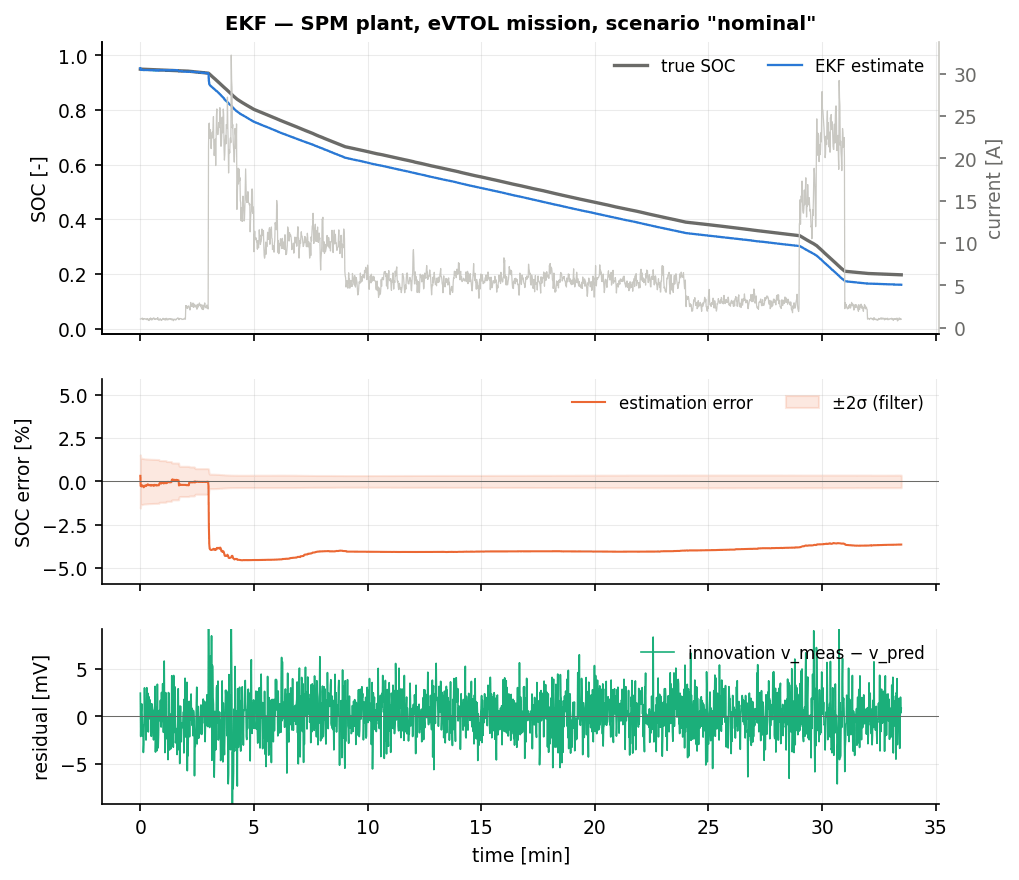
\includegraphics[width=\textwidth]{figures/cellspm_EKF_nominal.png}
\caption{EKF on the nominal mission with the electrochemical (SPM) plant. The estimate carries a persistent bias of about $4\,\%$ SOC even though the voltage residual stays at $1$\,mV.}
\end{figure}
The SPM block of the table is a different kind of test. The plant is the electrochemical
single-particle model; the estimator still runs a 2-RC equivalent circuit, fitted to that plant,
which leaves a \emph{structured} residual of about $4$\,mV (Butler--Volmer kinetics and
solid-phase diffusion that no 2-RC circuit can reproduce) and a slow second branch,
$\tau_2 = 556$\,s. Over a $33$-minute mission a $556$\,s pole barely relaxes, so $v_2(t)$ is
close to an affine ramp --- and so is $\ocv(\soc(t))$ while the cell discharges at a roughly
constant rate. The two channels through which the measurement sees the state,
$(\partial\ocv/\partial\soc)\,\delta\soc$ and $-\delta v_2$, are therefore nearly collinear in
the information accumulated over the flight: the pair $(\soc, v_2)$ is close to unobservable,
and no filter can decide whether a persistent few-millivolt residual belongs to the slow RC
branch or to the state of charge. Because that direction is weakly observable, a $4$\,mV
structured error maps onto \emph{several per cent} of SOC instead of the
$4\,\text{mV}/0.8\,\text{V}\approx0.5\,\%$ a well-conditioned channel would give. This
$(\soc,v_2)$ ambiguity, not the size of the residual, is the mechanism behind the
$3.7$--$4.6\,\%$ band in which the whole classical family sits.

The EKF sits at $3.73\,\%$ steady state on SPM \texttt{nominal} --- seventy times its ECM
figure --- while its voltage residual is only $1.02$\,mV, barely above the ECM value. That
combination is the signature of the ambiguity: the filter fits the voltage almost perfectly and
is nevertheless wrong about SOC by $4\,\%$, because it has paid for the fit with $v_2$ and
$\soc$ in the wrong proportion. Nothing diverges and $t_{\text{conv}} = 0$ everywhere (the
error is a bias, not a drift). \texttt{cold} is the worst case at $7.35\,\%$: at $0^\circ$C the
diffusion overpotential the ECM cannot represent is largest, and the $\tau_2$ branch is slower
still. \texttt{outliers} is, paradoxically, the \emph{best} SPM scenario ($1.99\,\%$): the
corrupted samples widen the effective innovation covariance and stop the filter committing so
hard to the ambiguous direction. Among the filters of this chapter's family the EKF is at the
good end of the band --- the tighter its linearisation, the less weight it puts on the badly
conditioned OCV channel --- and only the frozen-linearisation LKF (Chapter~\ref{ch:lkf},
$1.72\,\%$) and the second-order EKF ($3.52\,\%$) do better.

\section{Summary}
Use the EKF when the model is differentiable, the Jacobians are cheap and the prior is tight
relative to the curvature of $f$ and $h$; on the ECM plant that covers eleven of the twelve
scenarios at a cost of $0.44$--$0.48\,\SI{}{\micro\second}$ per step. Do not use it when a large
prior uncertainty meets a curved measurement function, because the first-order innovation
covariance \eqref{eq:ekf-S} will make the filter over-confident and lock in the error --- the
\texttt{combined} scenario is the object lesson. On a plant whose physics the ECM cannot
represent (the SPM rows) no amount of filtering fixes a $4\,\%$ bias that lives in a nearly
unobservable direction; that needs a better model or an augmented state, not a better filter.
If the same code has to survive a single-precision or fixed-point target, prefer the
algebraically identical U-D or square-root implementations; they cost nothing extra in accuracy
and remove the definiteness question entirely.
